\chapter{Déroulement}\thispagestyle{fancy}

\paragraph{}
Cette chapitre explique les travaux principale pendant mon stage. Il se compose de trois sections. Tous d'abord, j'ai installé et configuré un environnement de développement afin de améliorer l'efficacité. Ensuit, le travaille principale est l'amélioration du framework KdoMotiv Médium. Dernièrement, c'est quelque projets lesquels j'ai réalisé par KdoMotiv.

\section{Configuration de l'environnement}

\subsection{Installer un serveur linux local}
\paragraph{}
Comme le problème j'ai expliqué dans le chapitre avant, ce n'est pas très pratique avec un serveur disant sans droits ou un serveur local avec système exploitation de windows.
Auparavant, quand les collègue de pôle web avait le problème sur quelque site, ils doivent communiquer directement chez notre pôle. En plus, il n'y a rien de trace ou histoire sur le problème. 
Par conséquent, j'ai choisi un ordinateur qui n'est utilisé plus comme un nouveau serveur local. 

Lorsque ubuntu est un système d'exploitation intuitif et sécurisé, idéal pour les ordinateurs de bureau, les serveurs, les netbooks et les ordinateurs portables. En plus, Ubuntu est libre, gratuit, et est composé de logiciels qui le sont également.

J'ai décidé d'installer ubuntu serveur 10.04(LTS\footnote{Long Term Support}) sur serveur local.

\subsubsection{Partition}
En fait, comme le serveur local n'est pas très puissant,il a juste 2G de RAM de ce PC.  il faut l'attribuer 2G de swap. La partition de disque est comme la table suivant.

\begin{table}[htbp]
\centering
\begin{tabular}{ll}
  \toprule
  Partition & G\\
  \midrule
	/ & 30 \\ 
	\hline 
	swap & 2 \\ 
	\hline 
	/var & 10 \\ 
	\hline 
	/tmp & 5 \\ 
	\hline 
	/home & reste \\
  \bottomrule
\end{tabular}
 \caption{\label{tab:Partition du serveur}Partition du serveur}
\end{table}

\subsubsection{Installation de l'environnement LAMP + PhpMyAdmin}
LAMP est un acronyme désignant un ensemble de logiciels libres permettant de construire des serveurs de sites web. L'acronyme original se réfère aux logiciels suivants :
\begin{itemize}
\item[•] Linux 
\item[•] Apache 
\item[•] MySQL 
\item[•] PHP 
\end{itemize}
Sur ce serveur local, on a aussi besoin de debuger le site php ou développer quelque fonctions de php sert à traiter les données locales. Il faut configurer un environnement plus proche ou similaire que l'environnement LAMP sur serveur distant. Pourquoi mettre un environnement plus similaire que celui sur serveur production? Au cas où si on va déployer ce que on a développer sur serveur local, mais ne fonctionne pas sur serveur de production. 

D'ailleurs, afin de contrôler le serveur plus facilement, j'ai aussi installé le OPENSSH. Après cette étap, je peux faire tous les opérations sur ma poste avec PuTTY\footnote{PuTTY est un émulateur de terminal doublé d'un client pour les protocoles SSH, Telnet, rlogin, et TCP brut.}

Mais, il y a encore de un peu de problème de ce serveur. Tous d'abord, comme c'est un PC dans réseau local, on n'a pas fixer l'adresse IP de cette machine. S'il a éprouvé la situation de coupure d'électricité de week-end, et le serveur a redémarré automatiquement, l'adresse IP de cette machine serait changé à cause de DHCP. C'est-à-dire chaque fois, on doit informer à les autre département du changement de l'adresse IP de serveur local.

Ce n'est pas pratique. La solution sera fixé l'adresse ip depuis la configuration du routeur.



\subsubsection{Installation de Ruby on Rails et RedMine}
Comme le problème lequel j'ai déjà expliqué dans le chapitre avant, ce n'est pas pratique de communiquer entre différent pôle  et suivre ou tracer des bugs de tous les projets. 

Par conséquent, j'ai trouver deux applications web candidats qui sert à la gestion de projet. Une est RedMine qui est programmé par Ruby, l'autre est Trac qui est programmé par python. Finalement, j'ai fixé d'utiliser RedMine dû à son plus agréable interface.  

Vu que RedMine est une web application sous framework Ruby on Rails. Il faut configurer la framework de ROR sur serveur local. 

Après l'installation et la configuration du ROR, la mise en place de Redmine est simple. Suivi les instructions depuis le site officiel de Redmine, c'est simple de mettre en œuvre. 

Ensuite, j'ai déposé tous les projets actuels de Data-Gest afin de gérer et tracer sur RedMine. On peut aussi apercevoir les anomalies, les évolution, les assistances de chaque projet.
\begin{figure}[hbtp]
\center
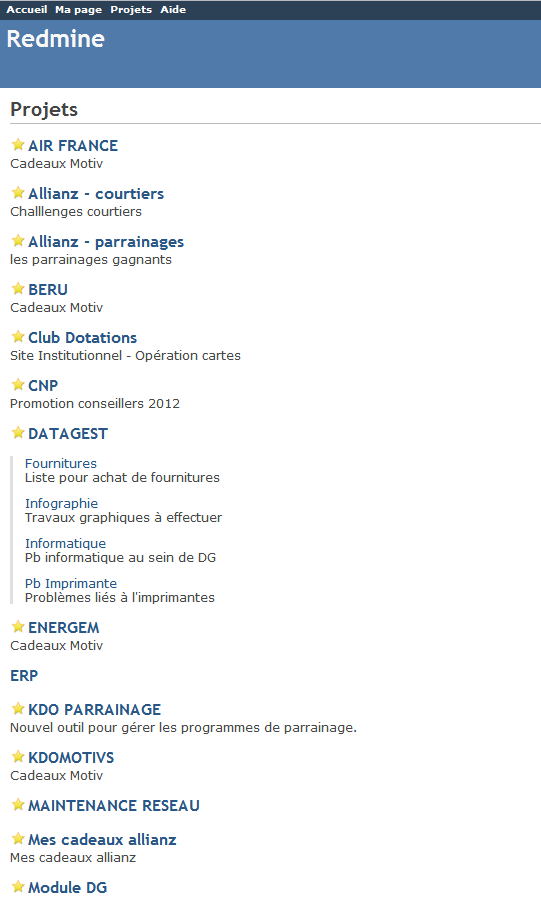
\includegraphics[width=10cm]{body/images/redmine-accueil.PNG}
\caption{Acceuil de Redmine}
\end{figure}



Cependant, quand j'ai essayé d'ajouter un ticket sur redmine à la fin du test, je n'ai reçu aucune  mail de notification lorsque le changement de ticket.

\subsubsection{Installation du serveur mail(Postfix) local}
Afin de fixer le problème que j'avais avant concernent le mails. J'ai installé le Postfix comme le serveur de messagerie électronique au remplacement du serveur \textbf{Sendmail}, vu qu'il est plus léger et plus stable. La configuration de Postfix en détail est dans annexe.

\subsubsection{Résume}
Étant donné que le serveur local peut juste être visité pas adresse IP, mais il y a plusieurs services sur ce serveur. Par conséquence, j'ai configuré les différent portes de Apache ou on peut y accéder pour utiliser le différent service. Par exemple, si on va accéder à PhpMyAdmin\footnote{Interface graphique pour gérer MySQL}, on peut juste ajout la porte correspondant après l'adresse IP.

\begin{table}[htbp]
\centering
\begin{tabular}{ll}
  \toprule
  Porte & Service\\
  \midrule
	80(Par défaut) & l'application RedMine \\ 
	 
	8080 & CMS Drupal, développement de site par Drupal \\ 
	 
	8888 & PhpMyAdmin, interface graphique pour la gestion Base de donnée \\ 
	 
  \bottomrule
\end{tabular}
 \caption{\label{tab:Service de différents portes}Service de différents portes}
\end{table}




\subsection{Configuration un serveur SVN sur seveur distant}

\subsection{Création de la documentation du Data-Gest}


\section{Amélioration du framework KdoMotiv}

\section{Projets}

